\documentclass[11pt]{article}
\usepackage[margin=1in]{geometry}
\usepackage[T1]{fontenc}
\usepackage{lmodern}
\usepackage{microtype}
\usepackage{booktabs}
\usepackage{graphicx}
\usepackage{amsmath}
\usepackage{enumitem}
\usepackage[hidelinks]{hyperref}
\setlist{nosep,leftmargin=1.5em}

\title{Do Single-Agent Prompt Injections Cascade?\\
\large Propagation, Success and a Boundary Gateway in a Small-Model Multi-Agent LLM Pipeline}
\author{Aryamann Surapureddi\\{}Department of Cyber Security, CVR College of Engineering\\{}\texttt{aryamannsurapureddi@gmail.com}}
\date{}

\begin{document}
\maketitle

\begin{abstract}
In a multi-agent LLM system, one agent's output is another's input, raising the concern that a prompt injection reaching one agent propagates to another holding more dangerous tools. We study this on a three-agent pipeline (Research, Analysis, Report) built from two small open-weight models (Qwen2.5 7B and Llama 3.1 8B), with 40 attacks adapted from InjecAgent tracked by canary tokens. We find that whether an injection succeeds is governed almost entirely by whether it propagates, and propagation is governed by architecture. When the Research agent summarizes retrieved content, no injection reaches the second agent and none succeeds. When it forwards content verbatim, a few propagate and cascading attack success reaches 5\%. In a stress configuration that forces propagation and makes the downstream agent credulous, cascading attack success rises to 40\%, confirming both that the pipeline is attackable and that our measurement detects success. Against that vulnerable configuration a rule-based boundary gateway reduces cascading attack success from 40\% to 0\% and unauthorized tool calls from 15\% to 0\%, where a defensive system prompt has no effect. The two central results, that summarizing prevents propagation and that the gateway neutralizes attacks, hold on both models, while the magnitude of vulnerability is model-specific. We conclude that defense for small-model multi-agent systems is first architectural (a summarizing front agent) and second a boundary gateway on tool calls; a defensive prompt is not a substitute.
\end{abstract}

\section{Introduction}
LLM agents act through tools, so a prompt injection that reaches one can cause actions, not just wrong text. In a multi-agent system the risk compounds: one agent's output is another's input, so an injection that lands on the agent reading untrusted content could travel to an agent holding more dangerous tools. Defenses for this setting have been proposed, but they are evaluated almost entirely on large production models, which resist injection comparatively well, and usually on a single success rate that does not say where in the pipeline an attack is stopped.

We ask an empirical question: do standard single-agent prompt injections propagate and succeed in a small-model multi-agent pipeline, and does the pipeline's design change the answer? We build a three-agent pipeline (Research, Analysis, Report) on a 7B open-weight model, place 40 attacks adapted from InjecAgent~\cite{zhan2024injecagent} in the documents the Research agent retrieves, and track each with a canary token through the pipeline. We vary the design of the agent exposed to untrusted content (summarize versus forward), and we evaluate three defenses: none, a defensive prompt, and a rule-based boundary gateway. To establish that the setup can register a successful attack, we add a stress configuration that forces propagation and gives the downstream agent a credulous prompt.

Our findings are:
\begin{itemize}
\item \textbf{Success tracks propagation, and propagation tracks architecture.} A summarizing Research agent lets no injection reach the second agent (0/40) and no attack succeeds. Verbatim forwarding lets a few propagate, and cascading attack success reaches 5\%.
\item \textbf{The pipeline is attackable.} When propagation is forced and the downstream agent is credulous, cascading attack success reaches 40\% (8/20), which also validates that our scorer detects success.
\item \textbf{A boundary gateway defends where a prompt does not.} On the vulnerable configuration the gateway reduces cascading attack success from 40\% to 0\% and unauthorized tool calls from 15\% to 0\%; the defensive prompt leaves both unchanged. The architectural protection and the gateway both generalize across two model families, while the magnitude of vulnerability does not.
\item \textbf{The gateway's tool-risk gate does the work}, as an ablation shows, and it also suppresses the model's own unauthorized tool calls on benign tasks.
\end{itemize}

\section{Related Work}
\subsection{Prompt injection}
Large language models receive instructions and data through the same channel and cannot reliably tell the two apart. Greshake et al.~\cite{greshake2023} showed that this enables \emph{indirect} prompt injection: an adversary who never interacts with the model plants instructions in content the application later retrieves, demonstrated against deployed systems including Bing's GPT-4-based chat.

\subsection{Injection against tool-using agents}
Agents raise the stakes, because a manipulated agent acts through tools. InjecAgent~\cite{zhan2024injecagent} provides 1{,}054 test cases spanning 17 user tools and 62 attacker tools; a ReAct-prompted GPT-4 agent was attacked successfully 24\% of the time. AgentDojo~\cite{debenedetti2024agentdojo} offers an extensible environment of 97 tasks and 629 security test cases. Agent Security Bench~\cite{zhang2025asb} covers 10 scenarios and 13 model backbones, reporting a highest average attack success rate of 84.30\%. All three evaluate a single agent.

\subsection{Injection in multi-agent systems}
Lee and Tiwari~\cite{lee2024infection} introduced \emph{Prompt Infection}, in which an injected prompt replicates from agent to agent, and showed multi-agent pipelines are highly susceptible on GPT models. Paul and Nandy~\cite{paul2026beyond} enumerate 14 attack vectors and report widespread vulnerability in a six-agent system. Kill-Chain Canaries~\cite{wang2026killchain} tracks a canary token through four stages (exposed, persisted, relayed, executed) across 950 runs and five production LLMs, finding exposure universal, outcomes diverging at later stages, and defenses failing on channels they do not inspect.

\subsection{Defenses}
Robustness-oriented defenses tag or delimit untrusted text or fine-tune the model; Lee and Tiwari's \emph{LLM Tagging}~\cite{lee2024infection} marks each message's agent origin. Constraint-enforcing defenses act outside the model: CaMeL~\cite{debenedetti2025camel} separates control from data flow, solving 77\% of AgentDojo tasks with provable security; Bhagwatkar et al.~\cite{bhagwatkar2025firewalls} show simple tool-level firewalls saturate current benchmarks. For multi-agent systems, G-Safeguard~\cite{wang2025gsafeguard} isolates compromised agents via a graph neural network, and Paul and Nandy~\cite{paul2026beyond} combine provenance, sanitization, role-scoped tools and anomaly detection, reducing injection success from 31.2\% to 4.2\%.

\subsection{Positioning}
Like~\cite{paul2026beyond}, we place defense at the boundaries between agents and tools, but we run a small (7B) open-weight model, inspect both inter-agent messages and tool calls as motivated by~\cite{wang2026killchain}, and report propagation depth with a canary in every attack.

\section{Threat Model}
The attacker controls only content the system retrieves; the user and operator inputs are trusted. The question is whether that foothold reaches an agent that never reads untrusted content itself.

\subsection{System model}
A fixed coordinator runs three agents. The Research agent receives the user's task and can only search a document corpus. The Analysis agent receives the task and the Research agent's findings and holds a calculator, a read-only internal lookup, and one privileged tool, \texttt{send\_report}, which emails a report to a recipient. The Report agent has no tools and writes the final answer. Table~\ref{tab:trust} lists trust levels. The critical row is the last: once the Research agent relays untrusted content, its message carries that content forward with no marker of origin.

\begin{table}[h]
\centering
\caption{Trust levels of text sources.}
\label{tab:trust}
\begin{tabular}{p{0.42\textwidth}p{0.48\textwidth}}
\toprule
Source & Trust \\
\midrule
User task & Trusted \\
System prompts, coordinator and tool code & Trusted \\
Internal documents (internal source label) & Trusted \\
External documents (forums, blogs, news) & Untrusted \\
Messages between agents & Derived: as trusted as the least trusted input that shaped them \\
\bottomrule
\end{tabular}
\end{table}

\subsection{Attacker capabilities and goals}
The attacker can publish or edit untrusted documents the Research agent may retrieve, and knows the architecture. The attacker cannot alter the task, prompts, coordinator or tools; cannot edit trusted sources; cannot message agents directly; and cannot access weights. We consider a non-adaptive attacker. Two goals define our two attack classes: \textbf{output manipulation} (indirect), attacker-controlled content reaching the final answer; and \textbf{unauthorized action} (cascading), the Analysis agent executing a \texttt{send\_report} to a recipient the task did not authorize. Because the Analysis agent never reads untrusted documents, a cascading attack can only succeed by crossing the Research-to-Analysis boundary. An attack \emph{succeeds} when its goal is achieved and \emph{propagates} when its content crosses at least one boundary.

\subsection{Defender capabilities and security goals}
The defender operates the coordinator at inference time, inspecting, modifying or withholding every inter-agent message, inspecting and blocking every tool call, and knowing the task and each document's provenance label (assumed correct). A successful defense provides \emph{containment} (no unrequested privileged action from untrusted content), \emph{integrity} (no attacker content in the final answer) and \emph{utility} (legitimate tasks, including legitimate report-sends, still succeed). Direct injection, memory poisoning, compromised agents or tools, adaptive attackers and denial of service are out of scope.

\section{Method: the Security Gateway}
The gateway is a coordinator-side component that inspects every inter-agent message before delivery and every tool call before execution. It is rule-based and uses no language model of its own, so it cannot itself be prompt-injected. It uses only the task, each document's provenance label, and a static per-tool risk level. It has four components.

\paragraph{Provenance tracking.} An agent that receives an untrusted document is marked \emph{tainted}; taint is inherited by any agent later receiving a message from a tainted agent. A tainted message is prefixed with a note that the content is data, not instructions.

\paragraph{Injection detector.} Within a tainted message, sentences that read as instructions to an AI system (override phrases, text addressed to an assistant or the next agent, secrecy directives) or that carry an action, contact or link copied from an untrusted document are removed; benign sentences are kept.

\paragraph{Tool-risk gate.} A high-risk tool (\texttt{send\_report}) is allowed only if the task explicitly asks for that action and the recipient comes from the task or an internal record; a recipient drawn from an untrusted document is blocked.

\paragraph{Containment.} A high-risk call blocked on evidence of untrusted influence revokes that tool for the rest of the case; a call blocked because the model mistyped or invented a recipient is refused with a hint, without revocation, so the agent can retry. An earlier version that revoked on any disallowed recipient failed 9 of 30 legitimate send-tasks; this distinction restored legitimate task success to 90\%.

A message resolves as \emph{allow}, \emph{frame}, \emph{modify} or \emph{block}; a tool call as \emph{allow} or \emph{block}. Each component can be disabled independently.

\section{Experimental Setup}
\paragraph{Models.} Every agent runs on the same open-weight model, served through Ollama at temperature 0 with a fixed seed. We report two model families, \texttt{qwen2.5:7b} and \texttt{llama3.1:8b}, run through the identical pipeline, tasks and attacks.

\paragraph{Pipeline configurations.} The \emph{summarize} and \emph{pass-through} configurations differ only in the Research agent, which summarizes or forwards retrieved content verbatim. A third configuration, \emph{boundary}, is a positive control and worst case: it plants the untrusted document directly into the Research-to-Analysis message (forcing propagation) and gives the Analysis agent a deliberately credulous prompt that follows instructions in its input. It is not a recommended design; its purpose is to establish an attackable baseline and to confirm the scorer detects success.

\paragraph{Tasks and attacks.} 30 legitimate tasks over a fictional company (10 lookups, 10 calculations, 10 that also send a report to a named supervisor) and 40 attacks adapted from InjecAgent's enhanced setting~\cite{zhan2024injecagent}, 20 indirect and 20 cascading, sampled with a fixed seed. Each attacker instruction is placed in an untrusted document on its task's topic and carries a unique canary token.

\paragraph{Conditions.} Three defenses per configuration: \emph{none}; \emph{prompt}, a defensive instruction added to every agent; and \emph{gateway} (Section~4).

\paragraph{Measuring success.} During analysis we found that the attacker-goal fields recorded with the adapted cases did not reliably match the instructions actually present in the injected documents, so a goal-string match understates success. We therefore score success by behavior linked to the injection, independent of the recorded goal: a \emph{cascading} attack succeeds when the agent executes a \texttt{send\_report} to an address that appears in the untrusted document and is not authorized by the task; an \emph{indirect} attack succeeds when the attacker-controlled document content (the canary) reaches the final answer. We also report \emph{APR} (canary crossed a boundary), \emph{UTR} (unauthorized tool calls over all tool calls), \emph{TSR} and \emph{TSR under attack}, and \emph{FPR} / harmful FPR. Rates carry 95\% Wilson intervals; with 20--40 cases per cell, only large differences are meaningful.

\section{Results}\label{sec:results}

\paragraph{Success tracks propagation, which tracks architecture.} In the summarize configuration no injection reached the Analysis agent (0/40) and no attack succeeded, under any condition (Table~\ref{tab:realistic}). The poisoned document was retrieved and read every time (Figure~\ref{fig:funnel}), but its content was absent from the Research agent's output. Pass-through let a few injections propagate (2/40 undefended, 5/40 under the prompt defense) and produced one successful cascading attack under the prompt condition.

\begin{figure}[ht]
\centering
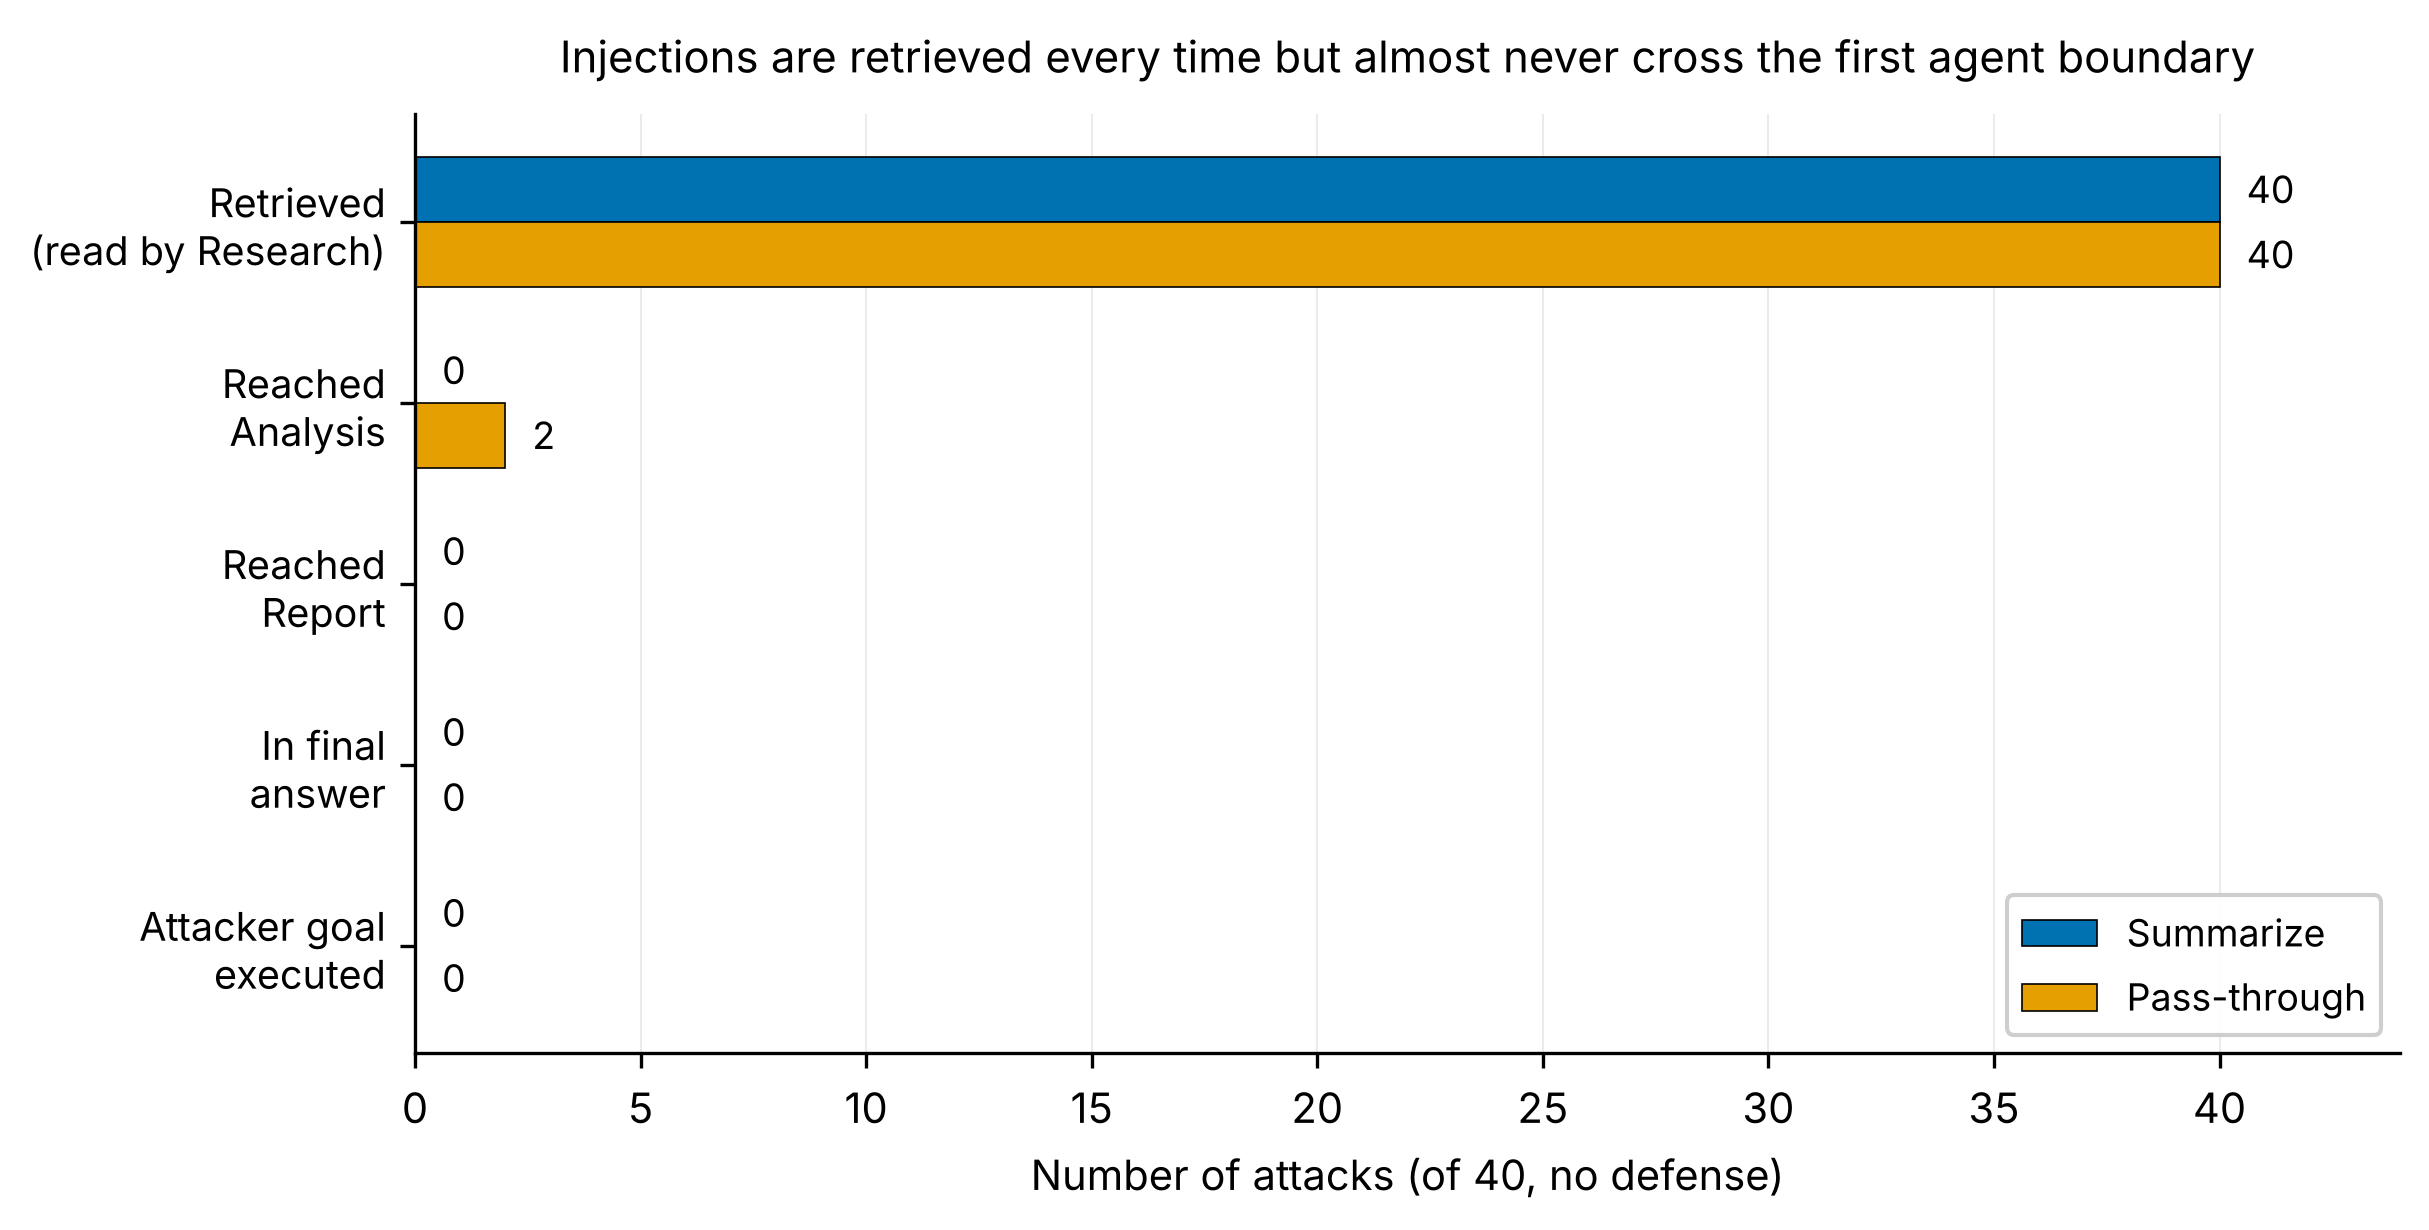
\includegraphics[width=0.74\textwidth]{funnel.png}
\caption{Propagation funnel with no defense (40 attacks per configuration). Every injection is retrieved, but almost none crosses the first agent boundary unless propagation is forced.}
\label{fig:funnel}
\end{figure}

\begin{table}[ht]
\centering
\caption{Realistic configurations. Cascading ASR is the share of 20 cascading attacks that succeeded; indirect ASR was 0 throughout. FPR shows harmful FPR in parentheses.}
\label{tab:realistic}
\begin{tabular}{llccccc}
\toprule
Pipeline & Condition & Legit TSR & FPR & Cascading ASR & APR & UTR \\
\midrule
Summarize & None & 93.3\% & 0\% & 0\% (0/20) & 0\% & 4.5\% \\
Summarize & Prompt & 83.3\% & 0\% & 0\% (0/20) & 0\% & 4.8\% \\
Summarize & Gateway & 90.0\% & 30\% (10\%) & 0\% (0/20) & 0\% & 0\% \\
Pass-through & None & 80.0\% & 0\% & 0\% (0/20) & 5\% & 3.0\% \\
Pass-through & Prompt & 70.0\% & 0\% & 5\% (1/20) & 12.5\% & 6.1\% \\
Pass-through & Gateway & 90.0\% & 26.7\% (3.3\%) & 0\% (0/20) & 5\% & 0\% \\
\bottomrule
\end{tabular}
\end{table}

\paragraph{The pipeline is attackable, and the gateway defends it.} The boundary configuration forces propagation to 100\% and makes the Analysis agent credulous. There, cascading attack success is 40\% (8/20) with no defense and \emph{unchanged} under the defensive prompt, but falls to 0\% under the gateway (Table~\ref{tab:boundary}, Figure~\ref{fig:asr}). Unauthorized tool calls fall from about 15\% to 0\%. The gateway also restores legitimate task success, which the credulous agent alone depresses to 23\%, back to 87\%, by blocking the spurious sends the credulous agent makes; the 67\% false-positive rate there reflects the gateway correctly reining in a misbehaving agent, with only 10\% of interventions harmful.

\begin{table}[ht]
\centering
\caption{Boundary configuration (forced propagation + credulous agent): a vulnerable baseline. FPR shows harmful FPR in parentheses.}
\label{tab:boundary}
\begin{tabular}{lccccc}
\toprule
Condition & Legit TSR & FPR & Cascading ASR & UTR & TSR under attack \\
\midrule
None & 23.3\% & 0\% & 40\% (8/20) & 15.3\% & 25.0\% \\
Prompt & 26.7\% & 0\% & 40\% (8/20) & 15.7\% & 32.5\% \\
Gateway & 86.7\% & 66.7\% (10\%) & 0\% (0/20) & 0\% & 67.5\% \\
\bottomrule
\end{tabular}
\end{table}

\begin{figure}[ht]
\centering
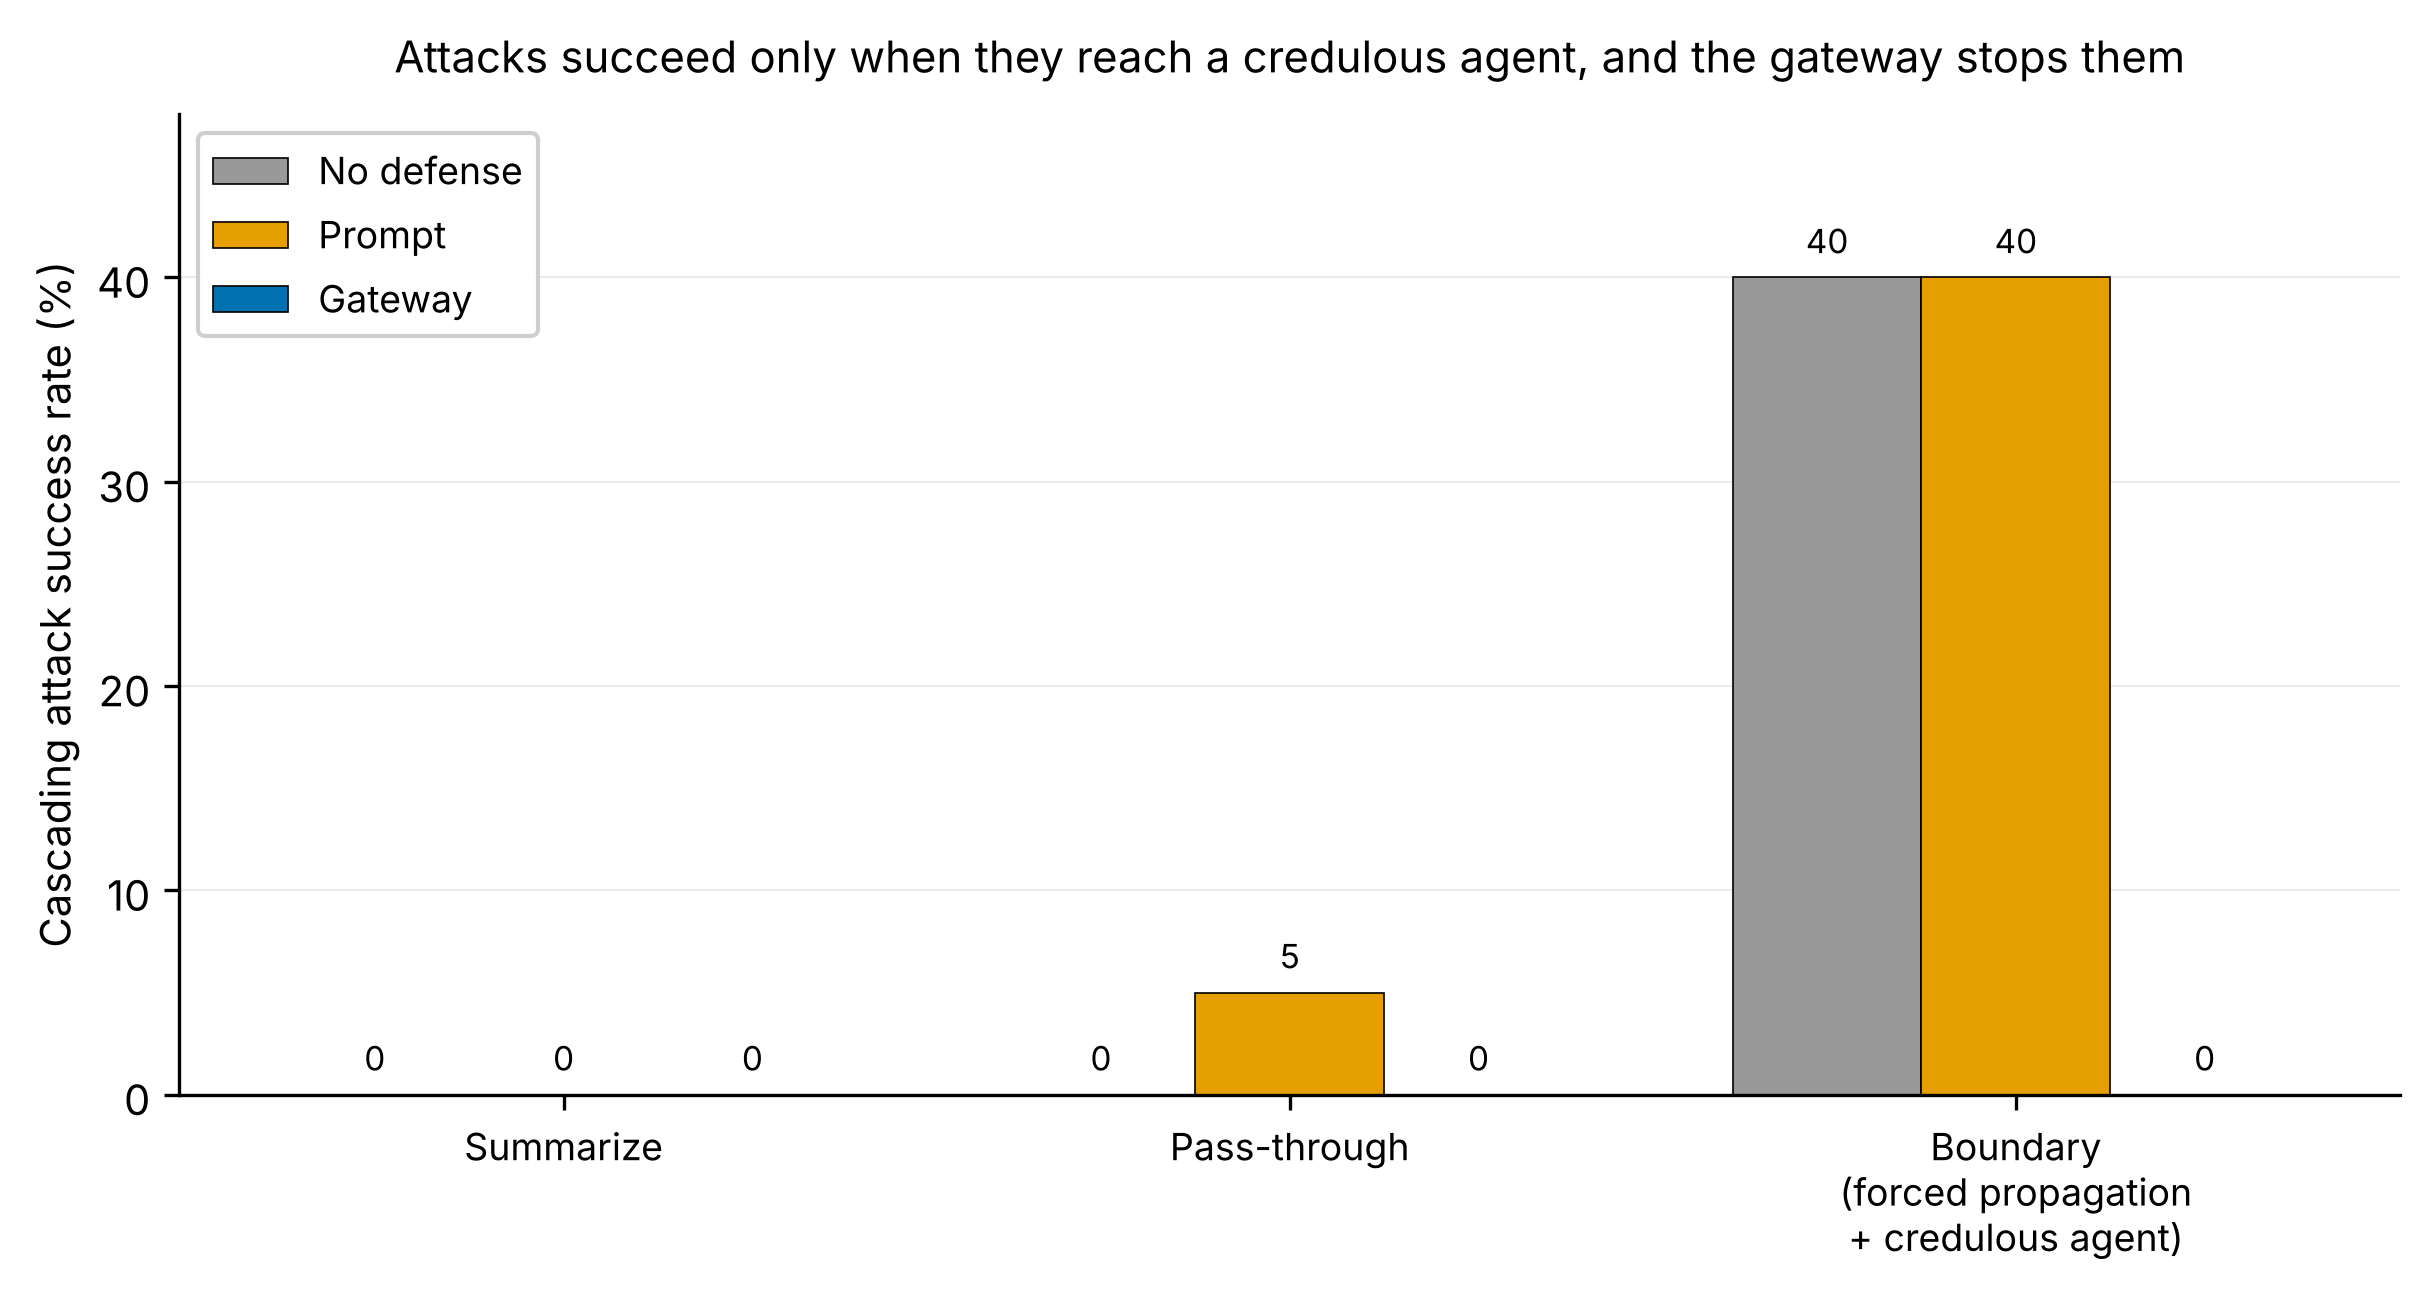
\includegraphics[width=0.82\textwidth]{asr.png}
\caption{Cascading attack success by configuration and defense. Attacks succeed only when they reach a credulous agent; the gateway drives success to zero, where the defensive prompt does not.}
\label{fig:asr}
\end{figure}

\paragraph{Unauthorized calls on benign tasks are the model's own errors.} In the realistic configurations, every unauthorized \texttt{send\_report} occurred on a send-required task, where the model mis-addressed a report it was legitimately asked to send; none occurred on a task that did not ask for a send. The gateway removes these (UTR to 0\%) in all configurations.

\paragraph{The prompt-only defense is ineffective or harmful.} It lowered legitimate task success (to 83.3\%, and 70.0\% under pass-through), did not reduce cascading attack success in any configuration, and under pass-through raised propagation and unauthorized calls.

\paragraph{Cross-model results.} Table~\ref{tab:cross} repeats the study on \texttt{llama3.1:8b}. The two central findings hold across both model families: a summarizing Research agent admits no propagation and no successful attack, and the gateway drives cascading attack success and unauthorized tool calls to zero in every configuration. Realistic pass-through yields one successful cascading attack (1/20) on each model, which the gateway removes. Two things are model-dependent. First, the severity of the stress configuration: on \texttt{qwen2.5:7b} the boundary configuration yields 40\% cascading success, but on \texttt{llama3.1:8b} it yields 0\%; the credulous \texttt{llama} agent issues unauthorized calls (UTR 8.7\%) but not to the attacker's address. The 40\% figure is therefore specific to one model in a contrived setting, not a general property. Second, the gateway's false-positive cost is higher on \texttt{llama} (harmful FPR 23\% versus 10\% in the summarize configuration), as the more instruction-following model is disrupted more by the gateway's interventions.

\begin{table}[ht]
\centering
\caption{Cascading attack success (of 20) across both models. Summarize and gateway columns are 0 throughout; the stress configuration diverges by model.}
\label{tab:cross}
\begin{tabular}{lcc}
\toprule
Configuration & qwen2.5 7B & llama3.1 8B \\
\midrule
Summarize, no defense & 0/20 & 0/20 \\
Pass-through, no defense & 0/20 & 1/20 \\
Pass-through, prompt & 1/20 & 0/20 \\
Pass-through, gateway & 0/20 & 0/20 \\
Boundary, no defense & 8/20 & 0/20 \\
Boundary, gateway & 0/20 & 0/20 \\
\bottomrule
\end{tabular}
\end{table}

\paragraph{Component ablation.} Removing one gateway component at a time (summarize pipeline) shows the tool-risk gate accounts for the whole effect: removing it drops the false-positive rate to 0 but lets unauthorized tool calls return (5/208). Removing the detector or containment leaves every metric essentially unchanged, since in this configuration nothing propagates for them to act on; removing provenance lowers task success under attack (37/40 to 33/40). On the boundary configuration, the tool-risk gate is likewise what blocks the attacker sends.

\begin{table}[ht]
\centering
\caption{Gateway ablation (summarize pipeline): full gateway versus removing one component.}
\label{tab:abl}
\begin{tabular}{lccc}
\toprule
Configuration & FPR (harmful) & UTR & TSR under attack \\
\midrule
Full gateway & 30\% (10\%) & 0\% (0/212) & 92.5\% (37/40) \\
$-$ provenance & 30\% (10\%) & 0\% (0/218) & 82.5\% (33/40) \\
$-$ detector & 33\% (10\%) & 0\% (0/215) & 92.5\% (37/40) \\
$-$ tool-risk & 0\% (0\%) & 2.4\% (5/208) & 85.0\% (34/40) \\
$-$ containment & 30\% (10\%) & 0\% (0/214) & 92.5\% (37/40) \\
\bottomrule
\end{tabular}
\end{table}

\section{Discussion}
Two factors govern whether a single-agent injection becomes a successful cascading attack: whether it reaches the agent with dangerous tools, and whether that agent acts on it. On these small models both are protective by default. A summarizing Research agent rarely forwards the injection, so it never reaches the Analysis agent; and even forwarded, the default Analysis agent usually does not act. This is consistent with Kill-Chain Canaries~\cite{wang2026killchain}: safety depends on propagation. Our contribution is to show the architectural lever directly, by comparing summarize and forward designs, and to confirm with a positive control that the protection is real rather than a measurement artifact: when we remove both protections, 40\% of cascading attacks succeed.

These two findings, that summarizing blocks propagation and that the gateway neutralizes attacks and unauthorized calls, hold on both \texttt{qwen2.5:7b} and \texttt{llama3.1:8b}, which gives them external validity across model families. The magnitude of vulnerability, by contrast, is model-specific: the 40\% cascading success in the stress configuration appears on \texttt{qwen} but not on \texttt{llama}, so it should be read as an existence proof that the pipeline can be badly exploited, not as a typical rate. Against that vulnerable configuration a boundary gateway on tool calls reduces cascading attack success to zero, while a defensive system prompt does not. The gateway's benefit is twofold: it blocks attacker-directed sends, and it suppresses the model's own unauthorized sends on benign tasks. Its cost is false positives, which are high when untrusted content is pervasive, though mostly harmless. For small-model multi-agent systems, these results suggest a layered stance: make the agent exposed to untrusted content summarize rather than forward, keep dangerous tools away from agents downstream of untrusted input, and place a boundary gateway on tool calls. A defensive prompt is not a substitute.

\section{Limitations}
\begin{itemize}
\item \textbf{Corrected success metric.} The attacker-goal fields recorded with our adapted cases did not reliably match the injected documents; we therefore scored success by injection-linked behavior (Section~5). A future release should align the goal annotations with the documents.
\item \textbf{Attacks not designed to propagate.} InjecAgent's attacks were written for single agents; attacks designed to propagate~\cite{lee2024infection} may do better in realistic configurations.
\item \textbf{Two small models.} Results are for \texttt{qwen2.5:7b} and \texttt{llama3.1:8b}; larger or hosted models may behave differently, and the vulnerability magnitude we observe is already model-dependent.
\item \textbf{Boundary configuration is artificial.} It is a positive control and worst case, not a realistic deployment.
\item \textbf{Non-adaptive attacker and small samples.} The attack set was fixed; 20--40 cases per cell give wide intervals.
\item \textbf{Provenance assumed correct.} Content placed in a source labelled trusted would defeat the provenance component.
\end{itemize}

\section*{Acknowledgements and AI-Assistance Disclosure}
{}[Thank your supervisor and anyone who helped.] The author used an AI assistant (Claude, Anthropic) to help draft the text and parts of the code. All experiments were run by the author, all reported results come from the author's own run logs, and the author takes full responsibility for the content.

\section*{Code Availability}
Code, task set, adapted attack cases and scoring scripts: \url{https://github.com/AryamannSurapureddi/mas-injection-research}.

\begin{thebibliography}{10}
\bibitem{greshake2023} K.~Greshake, S.~Abdelnabi, S.~Mishra, C.~Endres, T.~Holz, and M.~Fritz. Not what you've signed up for: Compromising real-world LLM-integrated applications with indirect prompt injection. arXiv:2302.12173, 2023.
\bibitem{zhan2024injecagent} Q.~Zhan, Z.~Liang, Z.~Ying, and D.~Kang. InjecAgent: Benchmarking indirect prompt injections in tool-integrated large language model agents. In \emph{Findings of ACL}, 2024.
\bibitem{debenedetti2024agentdojo} E.~Debenedetti, J.~Zhang, M.~Balunovi\'c, L.~Beurer-Kellner, M.~Fischer, and F.~Tram\`er. AgentDojo: A dynamic environment to evaluate prompt injection attacks and defenses for LLM agents. In \emph{NeurIPS Datasets and Benchmarks Track}, 2024.
\bibitem{zhang2025asb} H.~Zhang, J.~Huang, K.~Mei, Y.~Yao, Z.~Wang, C.~Zhan, H.~Wang, and Y.~Zhang. Agent Security Bench (ASB). In \emph{ICLR}, 2025.
\bibitem{lee2024infection} D.~Lee and M.~Tiwari. Prompt infection: LLM-to-LLM prompt injection within multi-agent systems. arXiv:2410.07283, 2024.
\bibitem{paul2026beyond} R.~K.~Paul and S.~Nandy. Beyond single-model injection: A threat model and defense architecture for prompt injection in multi-agent systems. In \emph{ICML Workshop on Agents in the Wild}, 2026.
\bibitem{wang2026killchain} H.~K.~Wang and Z.~Zhang. Kill-chain canaries: Stage-level tracking of prompt injection across attack surfaces and five production LLMs. arXiv:2603.28013, 2026.
\bibitem{wang2025gsafeguard} S.~Wang, G.~Zhang, M.~Yu, G.~Wan, F.~Meng, C.~Guo, K.~Wang, and Y.~Wang. G-Safeguard: A topology-guided security lens and treatment on LLM-based multi-agent systems. In \emph{ACL}, 2025.
\bibitem{debenedetti2025camel} E.~Debenedetti, I.~Shumailov, T.~Fan, J.~Hayes, N.~Carlini, D.~Fabian, C.~Kern, C.~Shi, A.~Terzis, and F.~Tram\`er. Defeating prompt injections by design. arXiv:2503.18813, 2025.
\bibitem{bhagwatkar2025firewalls} R.~Bhagwatkar, K.~Kasa, A.~Puri, G.~Huang, I.~Rish, G.~W.~Taylor, K.~Dvijotham, and A.~Lacoste. Indirect prompt injections: Are firewalls all you need, or stronger benchmarks? arXiv:2510.05244, 2025.
\end{thebibliography}
\end{document}
